\documentclass[a4paper, 12pt]{ctexart}
% generated by Madoko, version 1.1.3
%mdk-data-line={1}


\usepackage[heading-base={2},section-num={False},bib-label={hide},fontspec={True}]{madoko2}


\begin{document}



%mdk-data-line={6}
\mdxtitleblockstart{}
%mdk-data-line={6}
\mdxtitle{\mdline{6}数字媒体技术}%mdk
\mdtitleauthorrunning{}{}\mdxtitleblockend%mdk

%mdk-data-line={8}
\mdhr{}%mdk

%mdk-data-line={9}
\section{\mdline{9}1.\hspace*{0.5em}\mdline{9}PCA}\label{sec-pca}%mdk%mdk

%mdk-data-line={10}
\subsection{\mdline{10}1.1.\hspace*{0.5em}\mdline{10}背景:}\label{section}%mdk%mdk

%mdk-data-line={11}
\noindent\mdline{11}在多元统计分析中,主成分分析(英语:Principal components analysis,PCA)是一种分析、简化数据集的技术。主成分分析经常用于减少数据集的维数,同时保持数据集中的对方差贡献最大的特征。这是通过保留低阶主成分,忽略高阶主成分做到的。这样低阶成分往往能够保留住数据的最重要方面。但是,这也不是一定的,要视具体应用而定。由于主成分分析依赖所给数据,所以数据的准确性对分析结果影响很大。%mdk

%mdk-data-line={13}
\subsection{\mdline{13}1.2.\hspace*{0.5em}\mdline{13}数学定义:}\label{section}%mdk%mdk

%mdk-data-line={14}
\noindent\mdline{14}PCA的数学定义是:一个正交化线性变换,把数据变换到一个新的坐标系统中,使得这一数据的任何投影的第一大方差在第一个坐标(称为第一主成分)上,第二大方差在第二个坐标(第二主成分)上,依次类推\mdline{14}[4]\mdline{14}。
定义一个n × m的矩阵, XT为去平均值(以平均值为中心移动至原点)的数据,其行为数据样本,列为数据类别(注意,这里定义的是XT 而不是X)。则X的奇异值分解为X = WΣVT,其中m × m矩阵W是XXT的本征矢量矩阵, Σ是m × n的非负矩形对角矩阵,V是n × n的XTX的本征矢量矩阵。据此,%mdk

%mdk-data-line={18}
\mdline{18}\mdline{24}
\mdline{25}\mdline{25}
当 m \mdline{26}\textless{}\mdline{26} n − 1时,V 在通常情况下不是唯一定义的,而Y 则是唯一定义的。W 是一个正交矩阵,YT是XT的转置,且YT的第一列由第一主成分组成,第二列由第二主成分组成,依此类推。
为了得到一种降低数据维度的有效办法,我们可以利用WL把 X 映射到一个只应用前面L个向量的低维空间中去:%mdk


%mdk-data-line={88}
\noindent\mdline{88}X 的单向量矩阵W相当于协方差矩阵的本征矢量 C = X XT,\mdline{88}\mdline{88}
\mdline{89}\mdline{89}%mdk








%mdk-data-line={367}
\subsection{\mdline{367}1.3.\hspace*{0.5em}\mdline{367}算法实现一般过程:}\label{section}%mdk%mdk

%mdk-data-line={368}
\begin{enumerate}[noitemsep,topsep=\mdcompacttopsep]%mdk

%mdk-data-line={368}
\item\mdline{368}求平均值以及做normalization%mdk

%mdk-data-line={369}
\item\mdline{369}求协方差矩阵(Covariance Matrix)%mdk

%mdk-data-line={370}
\item\mdline{370}求协方差矩阵的特征根和特征向量%mdk

%mdk-data-line={371}
\item\mdline{371}选择主要成分(信息量)%mdk

%mdk-data-line={372}
\item\mdline{372}转化得到降维的数据%mdk
%mdk
\end{enumerate}%mdk

%mdk-data-line={374}
\subsection{\mdline{374}1.4.\hspace*{0.5em}\mdline{374}实验结果}\label{section}%mdk%mdk

%mdk-data-line={375}
\noindent\mdline{375}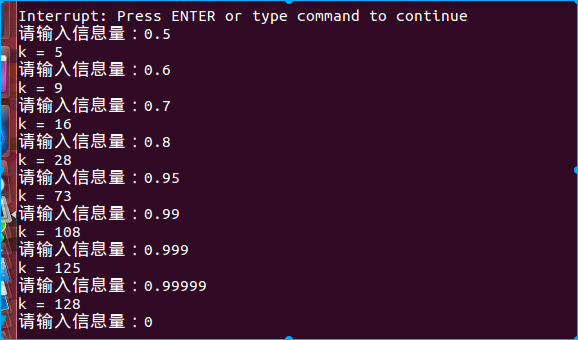
\includegraphics[keepaspectratio=true,width=\dimmin{}{\dimwidth{0.90}}]{images/PCA}{}\mdline{375}%mdk

%mdk-data-line={379}
\section{\mdline{379}2.\hspace*{0.5em}\mdline{379}JPEG压缩原理与DCT离散余弦变换}\label{sec-jpegdct}%mdk%mdk

%mdk-data-line={380}
\subsection{\mdline{380}2.1.\hspace*{0.5em}\mdline{380}背景:}\label{section}%mdk%mdk

%mdk-data-line={381}
\noindent\mdline{381}DCT变换的全称是离散余弦变换(Discrete Cosine Transform),主要用于将数据或图像的压缩,能够将空域的信号转换到频域上,具有良好的去相关性的性能。DCT变换本身是无损的,但是在图像编码等领域给接下来的量化、哈弗曼编码等创造了很好的条件,同时,由于DCT变换时对称的,所以,我们可以在量化编码后利用DCT反变换,在接收端恢复原始的图像信息。DCT变换在当前的图像分析已经压缩领域有着极为广大的用途,我们常见的JPEG静态图像编码以及MJPEG、MPEG动态编码等标准中都使用了DCT变换。%mdk

%mdk-data-line={383}
\mdline{383}\mdline{383}
\mdline{384} \mdline{384}%mdk

%mdk-data-line={386}
\subsection{\mdline{386}2.2.\hspace*{0.5em}\mdline{386}数学定义:}\label{section}%mdk%mdk

%mdk-data-line={388}
\subsubsection{\mdline{388}2.2.1.\hspace*{0.5em}\mdline{388}一维DCT变换}\label{sec-dct}%mdk%mdk

%mdk-data-line={389}
\noindent\mdline{389}一维DCT变换时二维DCT变换的基础,所以我们先来讨论下一维DCT变换。一维DCT变换共有8种形式,其中最常用的是第二种形式,
由于其运算简单、适用范围广。我们在这里只讨论这种形式,其表达式如下:%mdk

%mdk-data-line={393}
\mdline{393}\mdline{393}%mdk

%mdk-data-line={396}
\mdline{396}其中,f(i)为原始的信号,F(u)是DCT变换后的系数,N为原始信号的点可以认为是一个补偿系数,可以使DCT变换矩阵为正交矩阵。%mdk

%mdk-data-line={398}
\subsubsection{\mdline{398}2.2.2.\hspace*{0.5em}\mdline{398}二维DCT变换}\label{sec-dct}%mdk%mdk

%mdk-data-line={399}
\noindent\mdline{399}二维DCT变换其实是在一维DCT变换的基础上在做了一次DCT变换,其公式如下:%mdk

%mdk-data-line={401}
\mdline{401}\mdline{401}
\mdline{402}\mdline{402}
       由公式我们可以看出,上面只讨论了二维图像数据为方阵的情况,在实际应用中,如果不是方阵的数据一般都是补齐之后再做变换的,重构之后可以去掉补齐的部分,得到原始的图像信息,这个尝试一下,应该比较容易理解。%mdk

%mdk-data-line={405}
\mdline{405}另外,由于DCT变换高度的对称性,在使用Matlab进行相关的运算时,我们可以使用更简单的矩阵处理方式:%mdk

%mdk-data-line={407}
\mdline{407}\mdline{407}%mdk

%mdk-data-line={410}
\subsection{\mdline{410}2.3.\hspace*{0.5em}\mdline{410}JPEG压缩流程:}\label{sec-jpeg}%mdk%mdk

%mdk-data-line={411}
\begin{enumerate}[noitemsep,topsep=\mdcompacttopsep]%mdk

%mdk-data-line={411}
\item\mdline{411}以8x8的图象块为基本单位进行编码%mdk

%mdk-data-line={412}
\item\mdline{412}将RGB转换为亮度-色调-饱和度系统(YUV),并重新采样%mdk

%mdk-data-line={413}
\item\mdline{413}FDCT%mdk

%mdk-data-line={414}
\item\mdline{414}量化%mdk

%mdk-data-line={415}
\item\mdline{415}编码%mdk

%mdk-data-line={416}
\item\mdline{416}解码%mdk

%mdk-data-line={417}
\item\mdline{417}反量化%mdk

%mdk-data-line={418}
\item\mdline{418}IDCT%mdk

%mdk-data-line={419}
\item\mdline{419}图像拼接%mdk
%mdk
\end{enumerate}%mdk

%mdk-data-line={421}
\subsection{\mdline{421}2.4.\hspace*{0.5em}\mdline{421}实验结果:}\label{section}%mdk%mdk

%mdk-data-line={422}
\noindent\mdline{422}\textbf{DCT:}\mdline{422}\mdline{422}
\mdline{423}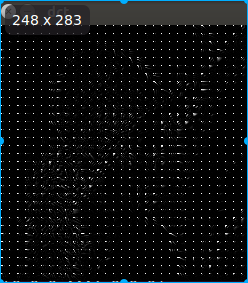
\includegraphics[keepaspectratio=true,width=\dimmin{}{\dimwidth{0.90}}]{images/dct}{}\mdline{423}%mdk

%mdk-data-line={425}
\noindent\mdline{425}\textbf{IDCT:}\mdline{425}\mdline{425}
\mdline{426}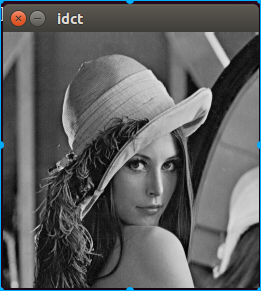
\includegraphics[keepaspectratio=true,width=\dimmin{}{\dimwidth{0.90}}]{images/idct}{}\mdline{426}%mdk

%mdk-data-line={430}
\noindent\mdline{430}\textbf{压缩率:10}\mdline{430}\mdline{430}
\mdline{431}\mdline{431}%mdk

%mdk-data-line={434}
\mdline{434}\mdline{434}
\mdline{435}\textbf{压缩率:50}\mdline{435}\mdline{435}
\mdline{436}\mdline{436}
\mdline{437}\mdline{437}
JPEG压缩比例,就是通过控制量化的多少来控制。比如,上面的量化矩阵Q,如果我把矩阵的每个数都double一下,那是不是会出现更多的0?!说不定都只有G(0, 0)非0,其他都是0,如果这样,那编码时就可以更省空间啦,N个0只要一个游程编码搞定,数据量超小。但也意味着,恢复时,会带来更多的误差,图像质量也会变差了。%mdk

%mdk-data-line={441}
\section{\mdline{441}3.\hspace*{0.5em}\mdline{441}Kmeans}\label{sec-kmeans}%mdk%mdk

%mdk-data-line={442}
\subsection{\mdline{442}3.1.\hspace*{0.5em}\mdline{442}背景}\label{section}%mdk%mdk

%mdk-data-line={443}
\noindent\mdline{443}k-平均算法源于信号处理中的一种向量量化方法,现在则更多地作为一种聚类分析方法流行于数据挖掘领域。k-平均聚类的目的是:把n个点(可以是样本的一次观察或一个实例)划分到k个聚类中,使得每个点都属于离他最近的均值(此即聚类中心)对应的聚类,以之作为聚类的标准。这个问题将归结为一个把数据空间划分为Voronoi cells的问题。
这个问题在计算上是困难的(NP困难),不过存在高效的启发式算法。一般情况下,都使用效率比较高的启发式算法,它们能够快速收敛于一个局部最优解。这些算法通常类似于通过迭代优化方法处理高斯混合分布的最大期望算法(EM算法)。而且,它们都使用聚类中心来为数据建模;然而k-平均聚类倾向于在可比较的空间范围内寻找聚类,期望-最大化技术却允许聚类有不同的形状。%mdk

%mdk-data-line={446}
\subsection{\mdline{446}3.2.\hspace*{0.5em}\mdline{446}数学定义}\label{section}%mdk%mdk

%mdk-data-line={447}
\noindent\mdline{447}设计的目的:使各个样本与所在簇的质心的均值的误差平方和达到最小(这也是评价K-means算法最后聚类效果的评价标准)。%mdk

%mdk-data-line={449}
\mdline{449}\mdline{449}%mdk

%mdk-data-line={452}
\subsection{\mdline{452}3.3.\hspace*{0.5em}\mdline{452}一般步骤}\label{section}%mdk%mdk

%mdk-data-line={454}
\begin{enumerate}[noitemsep,topsep=\mdcompacttopsep]%mdk

%mdk-data-line={454}
\item\mdline{454}创建k个点作为k个簇的起始质心(经常随机选择)。\mdline{454}\mdline{454}%mdk

%mdk-data-line={455}
\item\mdline{455}分别计算剩下的元素到k个簇中心的相异度(距离),将这些元素分别划归到相异度最低的簇。\mdline{455}\mdline{455}%mdk

%mdk-data-line={456}
\item\mdline{456}根据聚类结果,重新计算k个簇各自的中心,计算方法是取簇中所有元素各自维度的算术平均值。\mdline{456}\mdline{456}%mdk

%mdk-data-line={457}
\item\mdline{457}将D中全部元素按照新的中心重新聚类。\mdline{457}\mdline{457}%mdk

%mdk-data-line={458}
\item\mdline{458}重复第4步,直到聚类结果不再变化。\mdline{458}\mdline{458}%mdk
%mdk
\end{enumerate}%mdk

%mdk-data-line={462}
\subsection{\mdline{462}3.4.\hspace*{0.5em}\mdline{462}伪代码}\label{section}%mdk%mdk
\begin{mdpre}%mdk
\noindent~~创建k个点作为K个簇的起始质心(经常随机选择)\\
~~当任意一个点的蔟分配结果发生变化时(初始化为True)\\
~~~~~~~对数据集中的每个数据点,重新分配质心\\
~~~~~~~~~~~~对每个质心\\
~~~~~~~~~~~~~~~~~计算质心到数据点之间的距离\\
~~~~~~~~~~~~将数据点分配到距其最近的蔟\\
~~~~~~~对每个蔟,计算蔟中所有点的均值并将均值作为新的质心\\
%mdk
\end{mdpre}
%mdk-data-line={475}
\subsection{\mdline{475}3.5.\hspace*{0.5em}\mdline{475}实验结果}\label{section}%mdk%mdk

%mdk-data-line={476}
\noindent\mdline{476}由于数据作业所给数据集维数较高没法进行可视化,因此这里仅展示算法在二维数据下的可视化结果
数据集采用SIRI数据前两维%mdk

%mdk-data-line={479}
\mdline{479}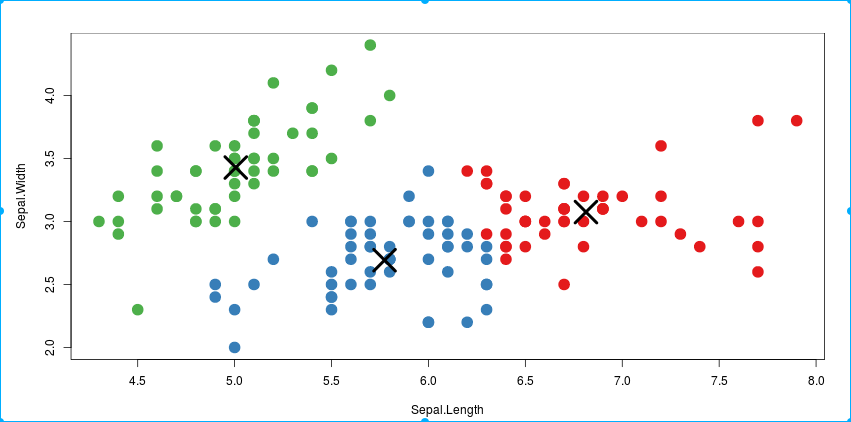
\includegraphics[keepaspectratio=true,width=\dimmin{}{\dimwidth{0.90}}]{images/kmeans}{}\mdline{479}%mdk

%mdk-data-line={482}
\section{\mdline{482}4.\hspace*{0.5em}\mdline{482}实验心得}\label{section}%mdk%mdk

%mdk-data-line={483}
\noindent\mdline{483}在本学期的数⼦媒体基础上机实验中,通过编写相应的程序,理解了 PCA 降维、DCT 变换
以及⾼维数据检索中的相关技术和其背后的原理。在信息爆炸性增长的时代,在这些信息中,多媒
体数据(图⽚、视频)占据了绝⼤部分,掌握如何对这些媒体信息进⾏检索、处理的技能是⼀项必
备的技能。熟悉了运用Python进项相关胆码的编写,大大简化了工作量。%mdk%mdk


\end{document}
